\documentclass[runningheads]{llncs}

\usepackage[T1]{fontenc}
\usepackage{graphicx}
\usepackage{placeins} % Ensures proper handling of \floatbarrier

\begin{document}

\title{Edge Computing in Cloud Computing}

\author{Galiléa LE MOULLEC (Mun ID: 202415993) \and Félicien MOQUET (Mun ID: 202415994)}
\authorrunning{G. Le Moullec, F. Moquet}
\institute{Memorial University of Newfoundland, St. John's, Canada\\
\email{glemoullec@mun.ca}, \email{fmoquet@mun.ca}}

\maketitle

\begin{abstract}
Edge computing significantly enhances cloud computing by localizing data processing near data sources, addressing bandwidth constraints, reducing latency, and improving real-time data analytics. This paper provides a detailed survey on edge computing, focusing on its principles, architecture, challenges, applications, and future trends.

\keywords{Edge Computing \and Cloud computing \and Challenges}
\end{abstract}

\section{Introduction}
Edge computing has emerged as a vital technology, complementing traditional cloud computing by bringing computation resources closer to data generation sources. Its goal is to reduce latency, optimize bandwidth, and enhance the efficiency of real-time applications, significantly impacting sectors such as autonomous vehicles, healthcare, and smart cities.

\subsection{Definition}
According to the Edge Computing Consortium (ECC), edge computing is a distributed computing paradigm that integrates networking, computing, storage, and application resources near data sources to provide intelligent services with minimal delay. By processing and storing data closer to its origin, edge computing minimizes latency, optimizes bandwidth usage, and enhances system responsiveness.



\subsection{Objectives of the Study}

The primary objective of this study is to explore how edge computing can effectively address and overcome existing limitations of traditional centralized cloud computing. Specifically, the research aims to analyze in detail how edge computing architectures, technologies, and methodologies can improve latency, enhance security, optimize network resources, and facilitate scalability in cloud-based systems. Furthermore, this study evaluates practical real-world use cases to illustrate concrete improvements enabled by edge computing. Finally, the study will outline future research directions, particularly the integration of edge computing with advanced technologies such as artificial intelligence (AI) and fifth-generation (5G) networks, demonstrating their combined potential to further enhance and expand cloud computing capabilities.


\section{Key Concepts of Edge Computing}
\subsection{Fundamental Principles}
Edge computing operates on decentralization, proximity, and real-time responsiveness principles. It significantly reduces data transit, optimizes latency, and improves data security by handling processing locally, closer to end-users and data generation sources.


\subsection{Architecture and Key Components}

\begin{figure}[ht]
    \centering
    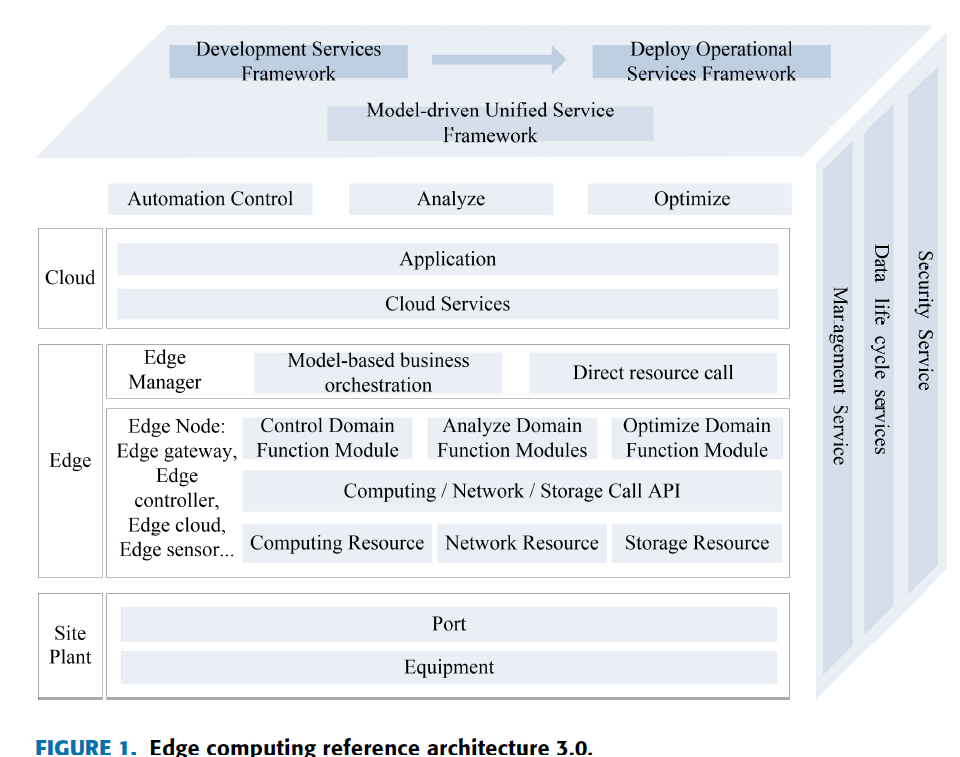
\includegraphics[width=0.85\textwidth]{IMG/6.png}
    \caption{Edge computing reference architecture 3.0}
    \label{fig:edge_reference_architecture}
    \end{figure}
\FloatBarrier


The general architecture of edge computing typically consists of three main hierarchical layers designed to efficiently manage data generation, processing, and analysis tasks. These layers are interconnected and cooperate closely to ensure optimal performance and responsiveness.


\subsubsection{Site Plant (Data Generation Layer)}
Edge devices represent the initial stage in the architecture, composed mainly of endpoints such as IoT sensors, actuators, smartphones, surveillance cameras, drones, wearable devices, and autonomous vehicles. These devices continuously generate data through their embedded sensors and are capable of basic local data preprocessing or filtering tasks. Their primary functions include:
\begin{itemize}
    \item Capturing real-time data from the physical environment.
    \item Performing simple preprocessing operations (e.g., noise reduction, data aggregation).
    \item Initial data validation and basic local decisions.
\end{itemize}

\subsubsection{Edge Layer (Local Processing Layer)}
Edge nodes are intermediate computing points located near edge devices, enabling localized data processing, efficient resource utilization, and reduced latency. These nodes bridge the gap between edge devices and cloud infrastructure, ensuring seamless data flow and intelligent decision-making. Positioned strategically close to data sources, they handle tasks such as advanced data filtering, aggregation, real-time analytics, and temporary data storage, reducing the need for constant cloud communication and minimizing network bandwidth consumption. Additionally, they serve as intermediaries that manage interactions between edge devices and cloud services, optimizing overall system performance. 

Several key components define the edge node layer. The \textbf{edge gateway} plays a crucial role in facilitating communication between edge devices and the cloud by handling protocol translation, network security, and initial data processing. It aggregates data from multiple sources, filtering redundant information and ensuring efficient transmission. Complementing this, the \textbf{edge controller} is responsible for real-time monitoring and automation, overseeing critical device-level operations such as industrial control systems, robotics, and smart infrastructure. By executing predefined logic, edge controllers enable immediate responses without relying on centralized processing.  

For more demanding computational tasks, the \textbf{edge cloud} functions as a localized micro data center, providing storage, processing power, and AI/ML capabilities closer to the source. This environment supports virtualization, distributed computing, and real-time analytics while ensuring low-latency execution. At the foundational level, \textbf{edge sensors} act as the primary data-generating components, capturing real-world information such as temperature, motion, video, and biometric data. Smart sensors with embedded processing capabilities can perform preliminary computations, such as anomaly detection and signal preprocessing, reducing unnecessary data transmission and improving efficiency.  

By leveraging these interconnected components, the local processing layer significantly enhances computational efficiency, ensures real-time analytics, and strengthens security by managing sensitive data closer to its origin.


\subsubsection{Cloud Layer (Centralized Processing Layer)}
Despite the strong local processing capabilities provided by edge nodes, some complex and resource-intensive analytical tasks still require central cloud resources. The hybrid architecture integrates edge nodes with traditional centralized cloud services to perform:
\begin{itemize}
    \item Deep learning, big data analytics, and extensive computational tasks.
    \item Centralized long-term data storage and historical data analysis.
    \item Global optimization and resource management.
    \item Comprehensive system management, updates, and coordination.
\end{itemize}

This integration ensures scalability, flexibility, and optimized resource allocation, combining the advantages of both centralized and decentralized computing models.

\subsubsection{Communication and Networking}
Communication within an edge computing architecture relies on a mix of wired and wireless protocols adapted to specific scenarios, including Ethernet, Wi-Fi, LTE, 5G, ZigBee, Bluetooth, and LoRa. Network communication is optimized for low latency, high reliability, and secure data exchange, ensuring efficient and seamless interoperability across all layers.



\subsection{Difference with Centralized Cloud Computing}

\begin{figure}[ht]
    \centering
    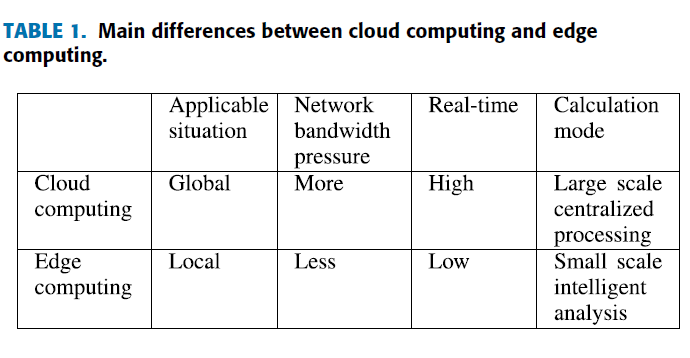
\includegraphics[width=0.7\textwidth]{IMG/5.png}
    \caption{Main differences between cloud computing and edge computing}
    \label{fig:cloud_vs_edge}
    \end{figure}
    \FloatBarrier



\subsubsection{Architectural Differences}
Centralized cloud computing utilizes a single or few data centers to handle all data processing and storage tasks. All data generated by end-users or devices is transmitted over the internet to these remote data centers for analysis and storage. In contrast, edge computing adopts a decentralized architecture, distributing computational resources close to the points of data generation. This distribution allows edge computing to handle data processing directly at the local nodes or devices.

\subsubsection{Latency and Real-Time Responsiveness}
In centralized cloud computing, latency is inherently high due to the distance between end-users and data centers, typically ranging from tens to hundreds of milliseconds, which can severely impact applications requiring immediate feedback. Edge computing significantly reduces latency by processing data locally, often achieving response times of only a few milliseconds, ideal for latency-sensitive applications such as autonomous vehicles, augmented reality, and real-time industrial monitoring.

\subsubsection{Bandwidth Utilization}
Centralized cloud computing often requires transmitting large volumes of data continuously, leading to substantial bandwidth consumption and network congestion. Conversely, edge computing processes most data locally and transmits only essential or aggregated information to the central cloud. This localized processing significantly reduces bandwidth usage and alleviates network loads.

\subsubsection{Data Security and Privacy}
Centralized cloud computing involves frequent transmission of data over public networks, increasing exposure to potential security breaches and data leaks. Edge computing enhances data security by reducing data transfers and handling sensitive information locally. Consequently, this approach minimizes the risks associated with network interception and centralized data breaches.

\subsubsection{Reliability and Fault Tolerance}
Reliability in centralized cloud computing heavily depends on the continuous availability of network connections and central servers, making services vulnerable to network disruptions or data center outages. Edge computing provides greater resilience due to its decentralized nature, enabling continuous operation of local systems even during external network disruptions, thereby enhancing fault tolerance.

\subsubsection{Energy Efficiency and Environmental Impact}
Centralized cloud infrastructures consume significant energy for data transmission, processing, and cooling systems in large data centers. Edge computing reduces energy consumption by limiting the transmission and central storage of massive data sets. By processing data locally, edge computing contributes to lower overall energy consumption and a reduced environmental footprint.




\section{Benefits for cloud computing and Challenges}

\begin{figure}[h!]
    \centering
    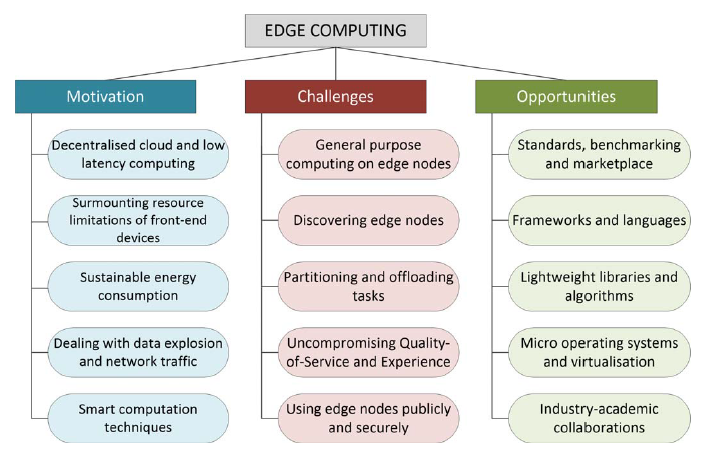
\includegraphics[width=0.85\textwidth]{IMG/10.png}
    \caption{Motivation, challenges and opportunities in edge computing}
    \label{fig:motivation_challenges_opportunities}
    \end{figure}
\FloatBarrier

\subsection{Limitations of Cloud Computing and the Advantages of Edge-Based Solutions}

Although traditional centralized cloud computing has revolutionized data processing and storage, it faces several critical limitations when applied to latency-sensitive, data-intensive, or privacy-critical scenarios. These inherent weaknesses hinder its performance in emerging domains such as autonomous systems, telemedicine, and large-scale IoT deployments. Edge computing emerges as a powerful complementary paradigm that directly addresses these challenges by relocating processing capabilities closer to the data source.

\subsubsection{Latency and Responsiveness}
Cloud computing typically introduces significant latency due to the physical distance between end-user devices and remote data centers. This delay is particularly detrimental for real-time applications requiring instantaneous decision-making, such as autonomous vehicles, augmented reality, and emergency response systems.

\noindent\textit{Edge Advantage:} By processing data locally or near the point of generation, edge computing drastically reduces round-trip time, enabling ultra-low latency responses. For instance, in autonomous driving, edge computing allows immediate obstacle recognition and reaction without relying on a remote server.

\subsubsection{Bandwidth Constraints and Network Congestion}

\begin{figure}[h!]
    \centering
    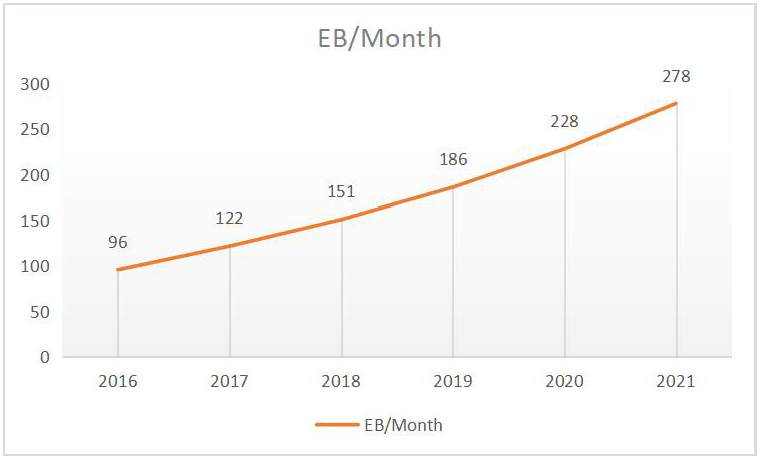
\includegraphics[width=0.75\textwidth]{IMG/8.png}
    \caption{Annual monthly average forecast of global internet traffic (EB/month)}
    \label{fig:internet_traffic}
\end{figure}
\FloatBarrier

With the exponential rise in IoT devices and connected systems, centralized cloud architectures increasingly struggle with bandwidth limitations and network congestion. Transmitting vast volumes of raw data to the cloud places enormous stress on existing infrastructure, driving up operational costs and increasing latency.

\noindent\textit{Edge Advantage:} Edge computing mitigates this issue by locally pre-processing data, transmitting only aggregated or critical information to central servers. This not only optimizes bandwidth usage but also ensures faster and more reliable service delivery. A typical example includes smart surveillance systems that analyze video streams locally and transmit only relevant segments.

\subsubsection{Security Risks and Privacy Concerns}
Transmitting sensitive data over public networks to centralized data centers elevates the risk of interception, unauthorized access, or regulatory non-compliance—particularly in fields such as healthcare or finance.

\noindent\textit{Edge Advantage:} Localized data processing enhances both privacy and security. Sensitive data can be processed and stored at the edge, reducing the frequency and scope of data transfers. This localized approach aligns more easily with data protection regulations like GDPR or HIPAA. For example, wearable medical devices using edge analytics can monitor patient vitals while keeping raw data secure on the device.

\subsubsection{Scalability Challenges}
Scaling a centralized cloud infrastructure often involves significant capital expenditure and long deployment cycles. Moreover, centralized models may struggle to adapt dynamically to large, dispersed networks of IoT or smart devices.

\noindent\textit{Edge Advantage:} The decentralized nature of edge computing enables horizontal scalability. New nodes can be deployed incrementally and independently, enhancing system flexibility without overloading central infrastructure. Industrial environments, for example, can scale analytics capabilities by simply adding edge modules to new machines.

\subsubsection{Reliability and Single-Point-of-Failure Risks}
Dependence on centralized data centers introduces single points of failure—if connectivity or the cloud server fails, the entire system may become inoperative.

\noindent\textit{Edge Advantage:} Edge architectures improve resilience by allowing local operations to continue even if central connectivity is lost. In manufacturing or remote monitoring scenarios, edge nodes ensure system continuity and data integrity despite intermittent cloud access.

\subsubsection{Energy Consumption and Operational Costs}
Large-scale cloud data centers require massive energy for processing, cooling, and data transmission, leading to high environmental and operational costs.

\noindent\textit{Edge Advantage:} By limiting unnecessary data transmission and enabling localized computing, edge systems reduce energy usage and improve operational efficiency. In IoT-based agriculture or smart building systems, edge devices can autonomously process sensor data, reducing dependency on energy-intensive cloud servers.

\bigskip

\noindent In summary, edge computing acts as a practical and scalable response to the limitations of centralized cloud computing. By enhancing latency, security, bandwidth, and resilience, edge technologies extend the reach and capability of the cloud, particularly for applications requiring local intelligence, real-time responsiveness, and high data autonomy.


\subsection{Challenges}

Despite its significant advantages, edge computing introduces several notable challenges that require careful consideration and management for successful deployment and operation.

\subsubsection{Managing Distributed Resources}
One of the core challenges of edge computing is the complexity involved in managing numerous distributed computing resources. Edge devices and nodes are geographically dispersed, and coordinating tasks such as resource allocation, load balancing, and efficient scheduling can be technically demanding. Managing consistent updates, synchronization, and data integrity across many decentralized nodes further increases complexity.

\noindent\textit{Example:} In smart city deployments, thousands of edge devices and sensors must be efficiently coordinated. Managing software updates, detecting failures promptly, and ensuring optimal distribution of computational tasks across all nodes require sophisticated resource management systems and algorithms.

\subsubsection{Security and Regulatory Compliance}
Decentralized data processing introduces additional security risks compared to centralized systems, as edge nodes and devices often lack the comprehensive security frameworks typical of centralized data centers. Ensuring data confidentiality, integrity, and availability across numerous edge devices can be challenging. Moreover, compliance with regulatory standards like GDPR or HIPAA becomes complex due to decentralized data storage and processing.

\noindent\textit{Example:} Medical IoT devices deployed in hospitals handle sensitive patient information locally. Ensuring compliance with privacy standards while maintaining robust security against data breaches requires comprehensive, multi-layered security measures across all edge devices.

\subsubsection{Interoperability with Cloud Computing}
Effective integration between decentralized edge systems and centralized cloud infrastructure remains a significant challenge. Seamless interoperability demands standardized protocols, data formats, and interfaces that facilitate smooth data exchange and cooperation between edge nodes and cloud services. Differences in hardware, software, and network standards further complicate integration.

\noindent\textit{Example:} Industrial IoT environments frequently involve devices from various manufacturers, each using different protocols. Establishing seamless integration between these diverse devices and a centralized cloud infrastructure necessitates adopting interoperable standards and middleware solutions such as EdgeX Foundry.

\subsubsection{Cost and Maintenance}
The initial deployment cost of edge computing infrastructure can be substantial. Edge computing involves numerous geographically dispersed hardware components, increasing upfront investment compared to centralized models. Ongoing maintenance and operational complexity add to long-term costs. Regular hardware upgrades, software updates, and system maintenance can become challenging due to the distributed nature of edge deployments.

\noindent\textit{Example:} Deploying a distributed edge computing network in remote areas, such as rural sensor networks for agriculture or environmental monitoring, requires significant initial capital investment for equipment installation. Moreover, ongoing operational costs, including routine hardware maintenance and software updates across dispersed locations, significantly impact total ownership costs.

\begin{figure}[ht]
    \centering
    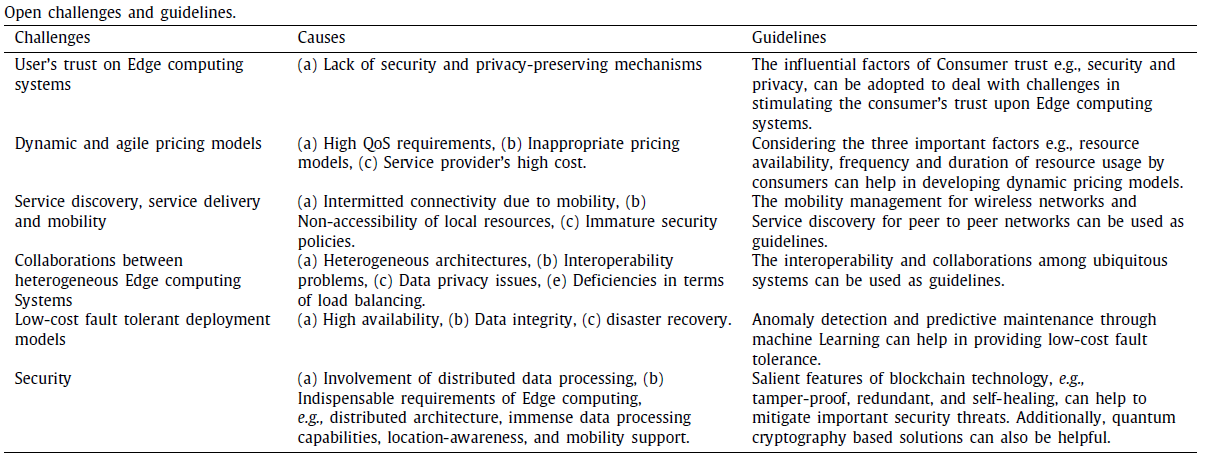
\includegraphics[width=\textwidth]{IMG/3.png}
    \caption{Open challenges and guidelines in edge computing}
    \label{fig:open_challenges_guidelines}
    \end{figure}
\FloatBarrier

\section{Applications and Use Cases}

\begin{figure}[ht]
    \centering
    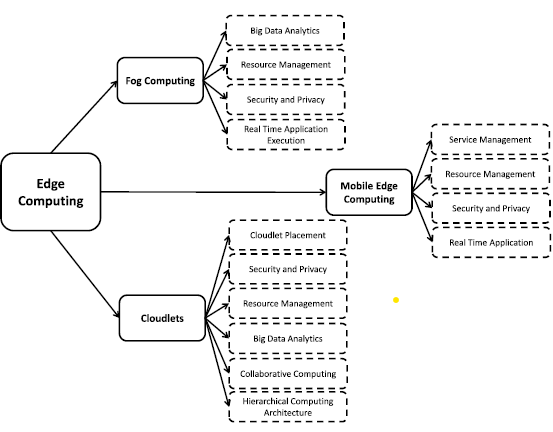
\includegraphics[width=0.75\textwidth]{IMG/1.png}
    \caption{Classifications of edge computing}
    \label{fig:edge_classifications}
    \end{figure}
\FloatBarrier

\subsection{Internet of Things (IoT)}

Edge computing has become a pivotal technology within IoT ecosystems by effectively addressing challenges such as latency, network congestion, data privacy, and scalability. It enhances the performance and security of IoT deployments across various sectors, notably in smart homes, industrial IoT, environmental monitoring, and wearable technologies.

\subsubsection{Real-Time Data Processing}
Edge computing facilitates real-time or near-real-time data analytics by enabling IoT devices and local nodes to process data immediately after generation. This capability is crucial in IoT applications where instant responsiveness is required to trigger actions or alerts based on real-time data.

\noindent\textit{Example:} In smart home environments, edge computing devices analyze sensor data such as motion, temperature, or humidity locally, enabling immediate responses. For example, a thermostat instantly adjusts the temperature upon detecting variations, significantly improving user comfort and energy efficiency.
\noindent\textbf{Case Study: Google Cloud Edge}
Google Cloud Edge enables real-time processing at distributed locations using AI and machine learning. For instance, Google Cloud IoT Edge integrates TensorFlow Lite to analyze sensor data locally, reducing the need for continuous cloud connectivity and enabling faster decision-making in applications like predictive maintenance and smart manufacturing.
\subsubsection{Enhanced Network Efficiency}
One of the critical advantages edge computing brings to IoT is enhanced network efficiency through local processing of massive amounts of IoT-generated data. By significantly reducing the amount of data transmitted to centralized clouds, edge computing alleviates network congestion and optimizes bandwidth usage, improving overall network performance.

\noindent\textit{Example:} Surveillance cameras integrated with edge computing technology perform video analytics directly on-site, transmitting only significant event alerts or summaries rather than continuous video streams. This approach reduces bandwidth consumption by over 80\%, greatly increasing network efficiency.
\noindent\textbf{Case Study: AWS Wavelength}
AWS Wavelength integrates computing services at the edge of 5G networks, allowing applications such as video streaming and AR/VR to process data locally, reducing latency and network congestion. 
\subsubsection{Improved Security and Privacy}
Edge computing significantly enhances security and privacy within IoT environments by reducing data exposure during network transit and allowing sensitive data to remain locally stored and processed. This minimizes the risk of data breaches or unauthorized access, essential for maintaining compliance with data protection regulations.

\noindent\textit{Example:} Wearable health monitoring devices use edge computing to locally process sensitive personal health data, such as heart rate or blood glucose levels. Data remains securely stored on the device or local gateway, transmitting only summarized or anonymized data to external servers, thus significantly enhancing privacy and security.
\noindent\textbf{Case Study: Microsoft Azure IoT Edge}
Azure IoT Edge allows healthcare applications to process patient data locally, ensuring compliance with HIPAA and other data protection laws. Hospitals leverage Azure IoT Edge to monitor patient vitals in real-time without continuously sending sensitive information to external cloud servers.
\subsubsection{Scalability and Reliability}
The decentralized nature of edge computing facilitates greater scalability and reliability for IoT systems. IoT networks can easily scale by integrating additional edge nodes or devices without extensive infrastructure modifications. Additionally, the distributed nature of edge computing increases system reliability, as local processing capabilities ensure uninterrupted service despite centralized server failures or network issues.

\noindent\textit{Example:} Agricultural IoT deployments, such as soil moisture and nutrient sensors, can quickly scale by adding new edge sensors without disrupting the existing system. Each sensor node independently processes data, providing continuous and reliable monitoring and control even if cloud connectivity is intermittently lost.
\noindent\textbf{Case Study: Cisco Edge Computing in Agriculture}
Cisco’s edge solutions enable precision agriculture by processing data from IoT sensors in real-time, optimizing irrigation and fertilization strategies. By reducing dependency on cloud connectivity, farms using Cisco’s technology improve yield predictions and resource management while ensuring continuous operation in remote areas.

\subsection{Autonomous Vehicles}

Edge computing plays a fundamental role in enabling the safe and efficient operation of autonomous vehicles by ensuring rapid processing of vast amounts of real-time sensor data. This decentralized computing approach significantly enhances responsiveness, decision-making precision, and operational safety.

\subsubsection{Real-Time Navigation and Decision-Making}
Autonomous vehicles generate substantial volumes of data through numerous onboard sensors, including LiDAR, radar, GPS, ultrasonic sensors, and cameras. Edge computing processes this data locally within the vehicle, allowing instantaneous navigation decisions without delays associated with data transmission to remote data centers.

\noindent\textit{Example:} An autonomous car approaching a busy intersection uses edge computing to immediately analyze sensor data and determine the appropriate speed, trajectory, and safe passage through traffic, ensuring precise and instantaneous navigational responses.

\noindent\textbf{Case Study: NVIDIA DRIVE}
NVIDIA DRIVE enables real-time AI processing within autonomous vehicles, allowing instant decision-making without reliance on cloud connectivity. By leveraging deep learning and computer vision at the edge, NVIDIA DRIVE enhances vehicle safety and operational efficiency, making autonomous driving more reliable in complex environments.

\subsubsection{Collision Avoidance and Safety Systems}
Safety-critical systems in autonomous vehicles rely heavily on the ultra-low latency processing provided by edge computing. Edge-enabled safety mechanisms swiftly identify potential collision scenarios and execute emergency maneuvers or alerts within milliseconds.

\noindent\textit{Example:} During highway driving, edge computing allows an autonomous vehicle to detect sudden obstacles, such as pedestrians or stalled cars, immediately triggering braking or evasive actions without depending on remote server decisions, thus preventing accidents.

\noindent\textbf{Case Study: Tesla Autopilot and FSD}
Tesla’s Full Self-Driving (FSD) system relies on edge computing to process camera and sensor data locally within the vehicle, enabling instant collision avoidance and autonomous navigation. By reducing dependency on external servers, Tesla enhances vehicle safety and real-time decision-making capabilities.

\subsubsection{Environmental and Contextual Analysis}
Edge computing enables continuous real-time analysis of complex environmental conditions around autonomous vehicles. Localized data processing supports accurate perception and contextual awareness, essential for adaptive decision-making in varied driving conditions.

\noindent\textit{Example:} Edge nodes analyze real-time data from weather sensors, road condition sensors, and surrounding vehicle data to dynamically adjust driving strategies (such as traction control or lane-keeping strategies), ensuring optimal vehicle behavior under changing environmental conditions.

\noindent\textbf{Case Study: Waymo's Edge AI}
Waymo employs edge AI to analyze environmental conditions, including road conditions, traffic signals, and pedestrian movements. This enables precise navigation decisions in real-time, allowing vehicles to adapt their driving behavior dynamically and ensuring safer autonomous driving experiences.
\subsubsection{Bandwidth Optimization and Data Reduction}
Due to the high volume of data generated by autonomous vehicles, centralized transmission to cloud servers can quickly saturate network bandwidth. Edge computing significantly reduces this data load by processing and analyzing sensor data locally, sending only essential information to central cloud servers.

\noindent\textit{Example:} Edge computing nodes within vehicles preprocess and compress video streams from onboard cameras, transmitting only critical data such as identified traffic violations or relevant road incidents to central monitoring platforms, thereby significantly decreasing bandwidth usage.

\noindent\textbf{Case Study: AWS Wavelength for Connected Vehicles}
AWS Wavelength integrates edge computing into 5G networks, enabling connected vehicles to process data locally and only transmit necessary insights. This reduces latency and enhances real-time vehicle communication for navigation and safety applications.


\subsubsection{Enhanced Reliability and Redundancy}
The decentralized nature of edge computing provides higher reliability and redundancy in autonomous vehicle systems. Local data processing reduces dependency on remote servers, ensuring continuous operation and maintaining vehicle safety even during network outages or data center failures.

\noindent\textit{Example:} In rural or remote driving scenarios where internet connectivity might be unreliable or intermittent, onboard edge computing ensures uninterrupted operational decision-making and navigation capabilities, maintaining vehicle safety and performance without dependence on continuous external connectivity.

\noindent\textbf{Case Study: Mobileye's Edge Vision Processing}
Mobileye integrates edge computing to process vision-based data locally, ensuring autonomous vehicles maintain real-time decision-making capabilities even in areas with poor network connectivity. This enhances reliability and safety, especially in remote or less-connected environments.

\subsection{Smart Cities and Intelligent Infrastructure}

Edge computing significantly transforms urban environments by enabling efficient, real-time management of infrastructure and resources. Its decentralized approach enhances responsiveness, security, and scalability, supporting diverse smart city applications such as traffic management, public safety, environmental monitoring, and resource optimization.

\subsubsection{Real-Time Traffic Management}
Edge computing allows local analysis of data from traffic sensors, cameras, and connected vehicles. It optimizes urban mobility by providing instantaneous decision-making capabilities that alleviate congestion, reduce travel time, and enhance safety.

\noindent\textit{Example:} Traffic lights equipped with edge computing analyze real-time traffic flow data at intersections, dynamically adjusting signal timings to minimize congestion, reducing waiting time by up to 30\%, and significantly improving overall urban mobility.

\noindent\textbf{Case Study: Siemens Smart Traffic Solutions}
Siemens employs edge computing in smart traffic management systems to optimize signal control and enhance urban mobility. By leveraging AI-driven analytics at the edge, Siemens solutions reduce congestion and improve traffic flow efficiency in major cities.

\subsubsection{Public Safety and Surveillance}
Edge computing enhances the effectiveness of urban surveillance systems by processing video feeds and sensor data locally, enabling rapid detection and response to incidents. Localized analysis ensures immediate recognition of potential threats or emergencies, enhancing public safety and responsiveness.

\noindent\textit{Example:} Surveillance cameras integrated with edge computing detect suspicious behavior (such as loitering, theft, or unauthorized access) instantly. Alerts are promptly sent to authorities, significantly reducing incident response times and improving city security.

\noindent\textbf{Case Study: Cisco Kinetic for Smart Cities}
Cisco Kinetic uses edge computing for smart city surveillance, analyzing real-time data from cameras and sensors to detect incidents instantly. This enables rapid response and improves urban security through intelligent threat detection.

\subsubsection{Resource Optimization and Management}
Edge computing supports smart city initiatives aimed at efficient resource utilization. Localized data processing enables dynamic management and distribution of resources such as energy, water, and waste management, leading to more sustainable and cost-effective urban operations.

\noindent\textit{Example:} Smart energy grids equipped with edge computing nodes monitor real-time energy consumption data across neighborhoods. These nodes automatically optimize energy distribution, quickly identifying and managing peaks in usage, thus significantly reducing waste and operational costs.

\subsubsection{Environmental Monitoring and Sustainability}
In smart cities, edge computing enhances environmental sustainability through local real-time monitoring and analysis of air quality, noise levels, and other environmental indicators. Immediate responses and alerts triggered by local nodes improve environmental management and public health outcomes.

\noindent\textit{Example:} Edge-enabled air quality sensors deployed throughout a city analyze pollution levels locally and generate immediate public alerts if hazardous conditions arise. Such real-time monitoring enables quicker corrective measures, such as traffic diversions or industrial emission controls, significantly improving air quality and urban health standards.

\subsubsection{Enhanced Connectivity and Communication}
Integration with advanced communication networks, such as 5G, allows edge computing to further improve connectivity in smart cities. It enables high-speed, low-latency communication between connected devices, supporting complex real-time urban applications.

\noindent\textit{Example:} 5G-enabled edge computing infrastructures facilitate real-time augmented reality (AR) applications for emergency services, providing firefighters or rescue teams immediate access to crucial environmental data, live video streams, and enhanced situational awareness, significantly improving operational effectiveness and safety.


\subsection{Industry and Manufacturing}

Edge computing revolutionizes industrial and manufacturing sectors by enabling rapid data analysis and local processing, significantly enhancing operational efficiency, reducing downtime, and facilitating intelligent automation. Its implementation leads to improved productivity, optimized resource use, and reduced operational costs.

\begin{figure}[ht]
    \centering
    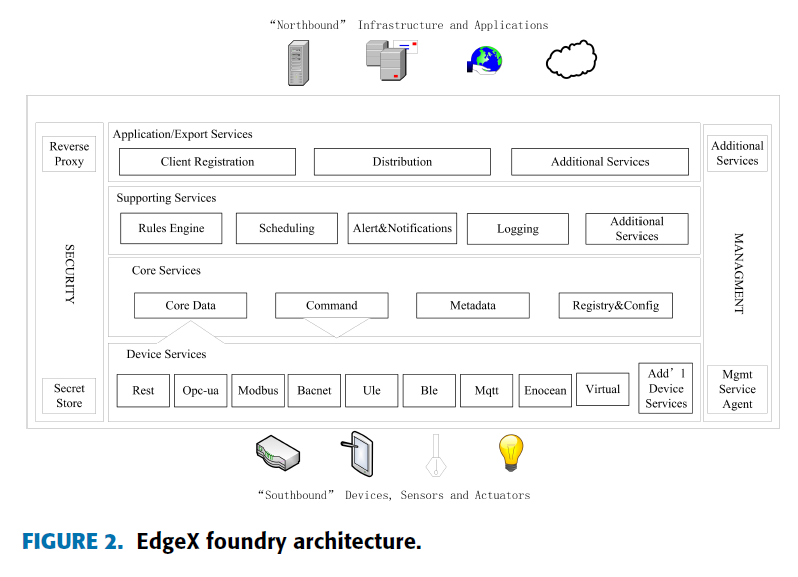
\includegraphics[width=0.8\textwidth]{IMG/7.png}
    \caption{EdgeX Foundry architecture}
    \label{fig:edgex_architecture}
    \end{figure}
\FloatBarrier
\subsubsection{Predictive Maintenance}
Edge computing provides real-time analytics capabilities that empower predictive maintenance practices. Local processing of sensor data enables immediate detection of equipment anomalies and early identification of potential failures, thereby reducing unscheduled downtime and maintenance costs.

\noindent\textit{Example:} In a manufacturing plant, edge devices continuously monitor the vibrations, temperature, and sound levels of industrial equipment. When anomalies are detected locally, alerts are immediately generated to perform maintenance proactively, reducing downtime by up to 50\% compared to traditional reactive methods.

\noindent\textbf{Case Study: Siemens MindSphere}
Siemens MindSphere leverages edge computing for industrial automation, predictive maintenance, and real-time data analytics. It enables manufacturers to process data locally, reducing downtime and optimizing production efficiency.

\subsubsection{Real-Time Data Analytics}
By enabling local data analytics directly at production sites, edge computing significantly enhances decision-making capabilities in industrial environments. Real-time insights from data streams allow manufacturers to rapidly adjust processes, optimize performance, and improve product quality.

\noindent\textit{Example:} On a production line, edge nodes analyze sensor data in real-time, identifying quality defects immediately. This capability allows manufacturers to adjust equipment parameters instantly, maintaining high-quality production standards and significantly reducing waste.

\subsubsection{Improved Operational Efficiency}
Edge computing enhances overall operational efficiency by automating real-time process monitoring and control. Localized processing ensures immediate responses to operational issues, thereby minimizing delays and enhancing throughput in production environments.

\noindent\textit{Example:} In automated assembly lines, edge computing continuously evaluates sensor data from robotic systems, immediately adjusting the robots' operations to optimize performance and efficiency. Such real-time adjustments can improve throughput and productivity by approximately 20–30\%.

\subsubsection{Enhanced Safety and Compliance}
Manufacturing environments require stringent adherence to safety standards and regulatory compliance. Edge computing facilitates rapid, local detection of hazardous conditions and immediate initiation of corrective actions, significantly improving workplace safety and compliance.

\noindent\textit{Example:} Edge-enabled safety sensors detect harmful chemical leaks or abnormal temperature increases immediately. Local edge nodes instantly trigger safety mechanisms, such as emergency shutdowns, ventilation adjustments, or automated fire suppression systems, ensuring worker safety and environmental compliance.

\subsubsection{Bandwidth Reduction and Network Optimization}
Edge computing reduces the dependency on central data centers by processing most data locally, significantly reducing the bandwidth required to transfer massive data volumes across the network. This localized data processing also reduces network congestion, ensuring smooth and uninterrupted manufacturing operations.

\noindent\textit{Example:} In a manufacturing environment with hundreds of IoT sensors, edge nodes perform local data aggregation and analysis. Instead of transmitting all raw data to centralized systems, only summarized insights or critical alerts are sent, reducing overall network traffic by up to 70–90\%.

\subsubsection{Flexibility and Scalability}
Edge computing provides manufacturing systems with enhanced flexibility and scalability. The decentralized nature of edge infrastructures simplifies the process of scaling operations by easily adding new nodes and equipment without major disruptions or significant costs.

\noindent\textit{Example:} A production facility experiencing growth can easily integrate additional edge nodes to manage increased data volumes and new equipment. This flexibility enables seamless expansion and adaptation to evolving production needs, reducing both the time and costs associated with scaling operations.


\subsection{Healthcare and Telemedicine}

Edge computing significantly enhances healthcare services and telemedicine by enabling rapid, localized data processing and analytics. It ensures real-time patient monitoring, immediate diagnostics, and swift medical interventions, contributing to improved patient outcomes, optimized healthcare delivery, and heightened data security.

\subsubsection{Real-Time Patient Monitoring}
Edge computing facilitates continuous, real-time monitoring of patient health data through medical IoT devices and wearable sensors. Local processing of vital health information ensures immediate detection of critical conditions, significantly reducing response times and potentially saving lives.

\noindent\textit{Example:} Wearable health monitoring devices, such as cardiac monitors, utilize edge computing to locally analyze patient data (e.g., heart rate, ECG signals). Immediate alerts are triggered if abnormal patterns or critical conditions such as arrhythmias are detected, enabling rapid interventions and enhancing patient safety.

\noindent\textbf{Case Study: GE Healthcare Edge AI}
GE Healthcare utilizes edge computing for real-time patient monitoring and diagnostics. By processing medical data locally, healthcare providers can receive instant insights, improving patient care and reducing treatment delays.

\subsubsection{Rapid and Accurate Diagnostics}
The decentralized nature of edge computing allows diagnostic procedures to be executed swiftly and locally, considerably reducing the time required for analysis and results. This capability is particularly advantageous in telemedicine scenarios, rural healthcare facilities, and emergency situations where immediate diagnosis is crucial.

\noindent\textit{Example:} Portable imaging devices such as ultrasound machines or X-ray units, integrated with edge computing, locally analyze imaging data using embedded artificial intelligence. Instant diagnostic results (such as detecting fractures or tumors) significantly accelerate clinical decision-making processes.

\subsubsection{Enhanced Emergency Medical Interventions}
In emergency medical situations, every second counts. Edge computing enables immediate local processing of critical patient data, ensuring prompt medical decisions and interventions, especially beneficial in ambulances, emergency rooms, and remote healthcare settings.

\noindent\textit{Example:} Ambulances equipped with edge computing devices analyze patient vital signs, such as oxygen saturation and blood pressure, in real-time during transit. These devices instantly communicate critical information and preliminary diagnostics directly to hospitals, significantly reducing treatment delays upon arrival.

\subsubsection{Data Privacy and Security}
Edge computing strengthens patient data privacy and security by minimizing the transmission of sensitive health information to centralized data centers. Localized data processing substantially reduces exposure risks during data transfer, ensuring compliance with strict healthcare regulations such as HIPAA or GDPR.

\noindent\textit{Example:} Patient health records processed locally by hospital edge computing nodes only transmit anonymized or securely encrypted data summaries to cloud-based analytics platforms. This strategy significantly mitigates potential risks associated with data breaches or unauthorized access.

\subsubsection{Improved Resource Management and Cost Efficiency}
Healthcare facilities benefit from optimized resource management and reduced costs through edge computing’s localized analytics and automation capabilities. Real-time insights enable better decision-making, improving operational efficiency, resource allocation, and patient flow management.

\noindent\textit{Example:} Hospitals equipped with edge nodes monitor real-time patient occupancy and resource utilization (such as beds, staff availability, and equipment usage). Immediate insights allow administrators to dynamically adjust resources, significantly reducing wait times, improving patient care quality, and lowering operational expenses.

\subsubsection{Support for Remote Healthcare and Telemedicine}
Edge computing supports telemedicine by ensuring high-quality, real-time video consultations, remote diagnostics, and patient monitoring. By processing data closer to patients, it delivers low-latency interactions critical for effective remote medical care.

\noindent\textit{Example:} In rural healthcare scenarios, edge-enabled telemedicine devices ensure real-time video consultations with specialists, rapid sharing of diagnostic information, and immediate local analytics. This approach significantly enhances healthcare accessibility and quality for remote or underserved populations.


\section{Trends and Future Perspectives}

\subsection{Technological Evolution and Innovation}

The effectiveness and scalability of edge computing continue to advance rapidly due to ongoing innovations across multiple technological dimensions. Significant progress in hardware capabilities, software intelligence, and networking technologies is enhancing the overall performance and applicability of edge computing systems.

\subsubsection{Advancements in Hardware Capabilities}
Continuous evolution in computing hardware, such as GPUs, CPUs, ASICs, and specialized edge processors, significantly improves local processing power, energy efficiency, and data handling capacity at the edge. This allows increasingly complex applications to run efficiently on edge nodes.

\noindent\textit{Example:} Development of low-power GPU accelerators, such as NVIDIA's Jetson platform or Google's Edge TPU, allows resource-intensive AI tasks (e.g., computer vision, deep learning inference) to be executed directly on edge devices with minimal energy consumption, enabling new use cases in real-time video analytics and robotics.

\subsubsection{Software and AI-driven Analytics}
Innovation in software, particularly artificial intelligence and machine learning algorithms tailored for resource-constrained environments, significantly increases the analytical capabilities of edge computing. AI-driven analytics algorithms optimized for edge computing enable faster, more accurate real-time data processing and predictive insights.

\noindent\textit{Example:} Edge-optimized neural network architectures (such as MobileNet, TinyML, and EfficientNet-lite) enable real-time analytics directly on mobile devices or IoT sensors, significantly reducing computational and memory footprints, thus facilitating advanced analytics capabilities even in constrained edge environments.

\subsubsection{Network Protocols and Communication Standards}
Ongoing innovations in networking and communication protocols significantly enhance connectivity, speed, and reliability in edge computing deployments. Advancements such as 5G, Wi-Fi 6, and low-power wide-area networks (LPWAN) allow edge nodes to communicate more efficiently and securely, supporting high-density device deployments.

\noindent\textit{Example:} The implementation of 5G networks enables ultra-low latency (below 1 ms) and increased device connectivity density, dramatically enhancing real-time responsiveness and enabling edge computing scenarios like smart transportation, augmented reality, and massive IoT deployments.

\subsubsection{Energy Efficiency and Power Management}
Technological advancements in power management and energy-efficient designs are crucial for extending the operational lifespan of edge devices, particularly in remote or battery-powered deployments. Improved battery technology, energy harvesting solutions, and power-efficient computation methods significantly enhance sustainability and reduce operational costs.

\noindent\textit{Example:} Energy harvesting technologies (solar, thermal, vibration-based) integrated with low-power edge processors allow sensor networks deployed in remote environmental monitoring scenarios to operate autonomously, reducing maintenance costs and enhancing sustainability.

\subsubsection{Containerization and Lightweight Virtualization}
Technological developments in software infrastructure, particularly lightweight virtualization and containerization technologies such as Docker and Kubernetes (K3s, MicroK8s), streamline deployment, maintenance, and scalability of edge computing applications, improving system flexibility and manageability.

\noindent\textit{Example:} Lightweight container orchestration frameworks like K3s enable efficient management and rapid deployment of containerized edge applications across thousands of nodes. This significantly simplifies software updates, improves reliability, and facilitates efficient resource utilization in large-scale edge deployments.

\subsubsection{Enhanced Security Innovations}
Ongoing technological innovation in cybersecurity, including embedded hardware security modules (HSMs), secure enclaves, and trusted execution environments (TEE), significantly enhances edge device security, protecting data privacy and system integrity against increasingly sophisticated threats.

\noindent\textit{Example:} Hardware-based security features, such as ARM's TrustZone and Intel's SGX, offer secure execution environments at the hardware level, ensuring sensitive data and computations remain protected from unauthorized access or tampering, significantly improving the overall security of edge deployments.


\subsection{Integration with Artificial Intelligence and 5G}


\begin{figure}[ht]
    \centering
    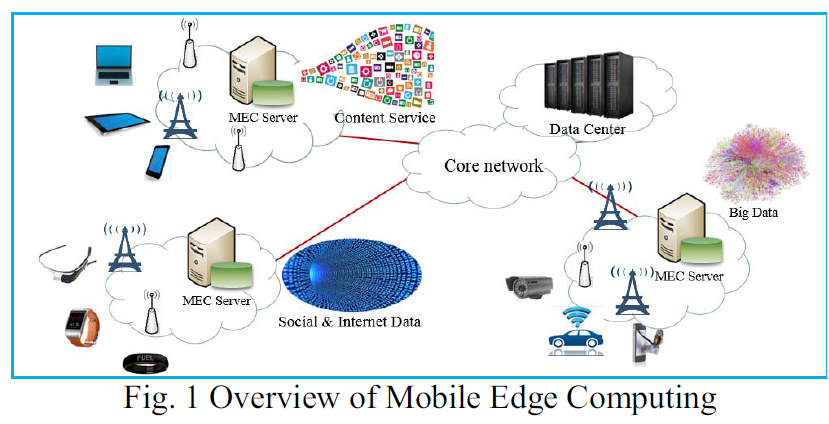
\includegraphics[width=0.8\textwidth]{IMG/4.png}
    \caption{General architecture of Mobile Edge Computing}
    \label{fig:mec_architecture}
    \end{figure}
\FloatBarrier

The convergence of edge computing, artificial intelligence (AI), and fifth-generation (5G) wireless technologies creates unprecedented opportunities for innovation. This integrated approach provides powerful analytics capabilities, ultra-low latency communications, and significantly increased bandwidth, enabling the emergence of advanced applications such as real-time augmented reality, smart robotics, and massive IoT systems.

\subsubsection{Enhanced Real-Time Analytics with AI}
Integrating AI with edge computing enables immediate local analysis and decision-making directly at the data source. This combination substantially improves the responsiveness, accuracy, and predictive capabilities of edge applications, facilitating intelligent automation and real-time data-driven insights.

\noindent\textit{Example:} In industrial automation, AI-driven edge nodes analyze data from machine sensors instantaneously, identifying operational anomalies or predicting equipment failures. Immediate actions triggered by these insights dramatically reduce downtime and improve productivity.

\subsubsection{Ultra-Low Latency Enabled by 5G}
The integration of edge computing with 5G technology significantly enhances network responsiveness, offering ultra-low latency data communication (often under 1 millisecond). This characteristic is crucial for latency-sensitive applications that require immediate data processing and response, ensuring seamless user experiences and real-time interactions.

\noindent\textit{Example:} Real-time augmented reality (AR) applications, powered by edge computing and 5G, provide instantaneous visual overlays and interactions without noticeable delays. In medical applications, AR-assisted surgeries rely on these low-latency characteristics for precision and accuracy.

\subsubsection{Massive IoT Deployments}
Edge computing combined with 5G and AI supports large-scale IoT implementations involving thousands or millions of interconnected devices. 5G networks facilitate significantly increased device density and high data throughput, while edge computing ensures local management and efficient processing of massive data volumes.

\noindent\textit{Example:} In smart city applications, massive IoT deployments utilizing edge computing, AI, and 5G networks allow thousands of sensors and connected devices to simultaneously transmit, process, and analyze data locally. Such large-scale implementations efficiently manage traffic, resource allocation, and public safety monitoring across vast urban areas.

\subsubsection{Intelligent Robotics and Automation}
AI-driven edge computing, supported by 5G connectivity, significantly advances robotic and automation systems. Robots gain immediate local processing capabilities, real-time decision-making, and advanced situational awareness, enabling intelligent and autonomous operation in dynamic environments.

\noindent\textit{Example:} Edge-enabled smart robots in manufacturing environments leverage AI algorithms to process visual data instantly, precisely navigating complex production environments, adapting to changing conditions, and performing intricate tasks without remote guidance delays.

\subsubsection{Bandwidth Optimization and Data Efficiency}
The combination of edge computing, AI, and 5G significantly optimizes bandwidth usage by analyzing and filtering data locally, transmitting only critical information over high-speed 5G networks. This approach considerably reduces network congestion and enhances overall system efficiency.

\noindent\textit{Example:} Autonomous vehicles use local AI-powered edge nodes to process vast sensor data streams instantly. Only critical event alerts or processed data are communicated through 5G networks to centralized cloud systems, drastically decreasing overall bandwidth consumption.

\subsubsection{Security and Privacy Enhancements}
AI-driven edge computing, integrated with secure 5G infrastructures, enhances data security and privacy. Localized data analytics minimize data transmission risks, while 5G provides robust security protocols, enabling secure and reliable data exchange.

\noindent\textit{Example:} Edge computing with AI-driven security analytics locally monitors traffic for anomalies or potential cyber threats. Supported by secure 5G network protocols, this local detection significantly improves cybersecurity defenses, protecting sensitive user data from unauthorized access or breaches.



\subsection{Research Challenges and Future Developments}

\begin{figure}[ht]
    \centering
    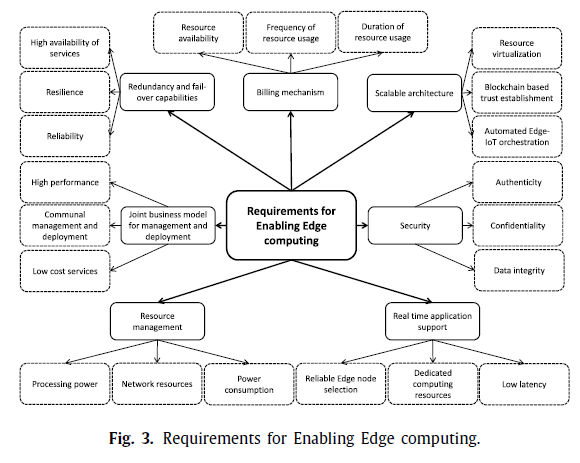
\includegraphics[width=0.8\textwidth]{IMG/2.png}
    \caption{Requirements for enabling edge computing}
    \label{fig:edge_requirements}
    \end{figure} 
\FloatBarrier

While edge computing has made substantial advances, significant research challenges remain. Addressing these challenges will enable broader adoption, improved performance, and enhanced capabilities across diverse industries. Prominent areas for future research include energy-efficient edge processing, advanced security and privacy solutions, standardized architecture models, and optimized cloud-edge integration.


\subsubsection{Energy-Efficient Edge Processing}
Energy efficiency is a critical research area, given the dispersed nature and limited resources of edge computing nodes and devices. Developing energy-aware processing algorithms, low-power hardware solutions, and optimized resource allocation strategies will significantly extend device lifetimes and reduce overall energy consumption.

\noindent\textit{Example:} Research efforts are focusing on creating ultra-low-power AI inference chips and energy-aware algorithms for edge devices, enabling extended operational periods for IoT sensors in remote or hard-to-access locations, such as environmental monitoring in forests or oceanographic sensors.

\subsubsection{Enhanced Security and Privacy Frameworks}
Improving security and privacy in decentralized edge computing environments remains a high-priority challenge. Research must develop comprehensive security models, advanced encryption techniques, secure communication protocols, and robust privacy-preserving mechanisms that protect data across heterogeneous and distributed edge nodes.

\noindent\textit{Example:} Future frameworks could include advanced federated learning approaches at edge nodes, where data remains local, reducing exposure risks. Enhanced cryptographic techniques, such as homomorphic encryption, could also be leveraged for secure, privacy-preserving edge analytics.

\subsubsection{Standardized Architecture Models}
A critical ongoing research area is the establishment of standardized architectural models, protocols, and interfaces. Unified standards facilitate interoperability among diverse devices, edge nodes, and cloud services, significantly simplifying deployment, integration, and scalability.

\noindent\textit{Example:} Initiatives like EdgeX Foundry and ETSI Multi-access Edge Computing (MEC) are creating standardized open-source platforms and guidelines that future research could extend. This ensures seamless integration across various vendor devices and cloud solutions, enabling easier implementation and broader adoption of edge computing.

\subsubsection{Improved Cloud-Edge Collaboration Mechanisms}
Optimizing the collaboration between edge nodes and centralized cloud computing infrastructures remains an important research challenge. Enhanced mechanisms for workload distribution, adaptive resource allocation, data synchronization, and efficient decision-making across edge and cloud platforms will greatly enhance system performance and reliability.

\noindent\textit{Example:} Research is exploring hybrid architectures that dynamically adjust the distribution of processing tasks based on real-time resource availability, network conditions, and application requirements. Developing smart middleware systems and automated orchestration tools can further improve cloud-edge cooperation and resource management.

\subsubsection{Scalable and Adaptive Edge Solutions}
Developing highly scalable and adaptive solutions that seamlessly accommodate growing numbers of edge nodes and diverse application demands is essential. Future research should focus on creating dynamically adaptive systems capable of self-organizing and self-optimizing based on changing operational conditions and network loads.

\noindent\textit{Example:} Autonomous, adaptive edge systems leveraging AI-based resource management can dynamically reconfigure their operations based on workload fluctuations or network disruptions, ensuring uninterrupted, optimized service provision in applications like smart grids and disaster-response scenarios.

\subsubsection{Integration with Emerging Technologies}
Future research must also explore deeper integration with emerging technologies such as quantum computing, blockchain, and next-generation communication protocols. Leveraging these technologies can offer enhanced computational capabilities, stronger security measures, and more efficient resource allocation strategies in edge computing environments.

\noindent\textit{Example:} Blockchain-based decentralized edge networks can improve trust, transparency, and security for distributed edge nodes, facilitating secure transactions and data sharing across diverse stakeholders in environments such as healthcare systems or supply chain management.

\section{Conclusion}
\subsection{Importance of Edge Computing in the Evolution of Cloud Computing}

Edge computing represents a fundamental evolution in the field of cloud computing by directly addressing and overcoming inherent limitations of traditional centralized cloud architectures. By shifting data processing closer to data sources, edge computing significantly reduces latency, a critical factor for real-time applications like autonomous vehicles, telemedicine, and augmented reality. Furthermore, it optimizes network resources by reducing bandwidth requirements and network congestion


\subsection{Growth and Research Perspectives}

The rapid technological advancements in edge computing, particularly when combined with emerging technologies such as artificial intelligence (AI) and fifth-generation (5G) networks, promise significant opportunities for further innovation and research. Future growth areas include developing highly efficient, intelligent, and adaptive edge processing algorithms capable of autonomously optimizing resource allocation and data analytics at local nodes.

Research will increasingly focus on addressing the remaining challenges in security, privacy, energy efficiency, and interoperability, establishing robust frameworks and standardized architectures for seamless cloud-edge collaboration. Emerging research topics such as federated learning at the edge, blockchain-based secure data sharing, and quantum computing integration will further drive innovation, enabling new applications and use cases.

Moreover, as edge computing gains widespread adoption across diverse sectors—
including healthcare, manufacturing, transportation, smart cities, and environmental monitoring—continuous improvements in technology will accelerate economic benefits, improve societal outcomes, and foster sustainable development. These developments position edge computing not only as a critical component of the future computing landscape but also as a fertile ground for multidisciplinary research and substantial industrial growth.

\section{References}
\nocite{*} % Include all entries from the .bib file, even if not cited
\bibliographystyle{splncs04} % Use the LNCS bibliography style
\bibliography{references}    % Replace 'references' with the name of your .bib file (without the .bib extension)



\end{document}
